\section{Usage}%
\label{sec:usage-examples:esdm-usage}
This section illustrated how ESDM can be used with different programming languages and tools.
The applications with NetCDF support don't need to be changed or recompiled as long as they are linked against the shared netcdf library.
They can simply use the ESDM-NetCDF version and benefit of ESDM.
To force them to use the ESDM-NetCDF version, the library can be pre-loaded by \lstinline|LD_PRELOAD| environment variable.

\subsection{NetCDF}%
\label{sec:usage-examples:netcdf}

NetCDF (Network Common Data Form)~\cite{netcdf2021} is a set of software libraries and machine-independent data formats that support the creation, access, and sharing of array-oriented scientific data. 
In particular, NetCDF is widely used in climate research.

The following examples write and read data to/from a NetCDF file.
(For simplicity, we omitted the error handling.)

The write example (\lstinline|./write|) creates a two dimensional variable in the \lstinline|esdm://data.nc| file.

\begin{preserve}
\lstinputlisting[language=c]{\examplespath/c/netcdf/write.c}
\end{preserve}

The read example (\lstinline|./read|) reads this variable.

\begin{preserve}
\lstinputlisting[language=c]{\examplespath/c/netcdf/read.c}
\end{preserve}

For a successful run ESDM requires three things.
Firstly, the \lstinline|esdm.conf| file must be located in the search path.
In this case, it is the current directory.
Secondly, ESDM requires an initialized ESDM directory structure.
If not existing, it can be created by the \lstinline|mkfs.esdm| tool.
Thirdly, files need to be prefixed with \lstinline|esdm://|.
This prefix is an indicator to the NetCDF library to redirect data to ESDM.
Otherwise, NetCDF will work as usual and create an \lstinline|*.nc| file.

The following script initialize the ESDM directory structure and runs the two examples.
\begin{preserve}
\lstinputlisting[language=c]{\examplespath/c/netcdf/run.sh}
\end{preserve}

Currently, ESDM does not provide a full compatibility to NetCDF.
The NetCDF compatibility is documented in the report released in \url{https://github.com/ESiWACE/esdm-netcdf/blob/master/libsrcesdm_test/report/report.pdf}.


\subsection{CDO}%
\label{sec:usage-examples:cdo}

The Climate Data Operator (CDO) software is a collection of many operators for standard processing of climate and forecast model data. 
The operators include simple statistical and arithmetic functions, data selection and subsampling tools, and spatial interpolation. 
CDO was developed to have the same set of processing functions for GRIB and NetCDF datasets in one package. 
The Climate Data Interface [CDI] is used for the fast and file format independent access to GRIB and NetCDF datasets. 
To enable ESDM, the files need the \lstinline|esdm://| prefix.
In the  example data is converted from GRIP to NetCDF format and written by ESDM according to the configuration in the \lstinline|esdm.conf| file.
%#cdo -f nc -copy data.grb esdm://data.nc 

\begin{preserve}
\lstinputlisting[language=c]{\examplespath/cdo/convert.sh}
\end{preserve}

%%cdo -selname,var1 data.nc esdm://data_x.nc
%In the second example CDO copies the variable \lstinline|var1| from \lstinline|data.nc| in \lstinline|esdm://data_x.nc| container.
%\begin{preserve}
%\lstinputlisting[language=c]{\examplespath/cdo/selection.sh}
%\end{preserve}

\subsection{XIOS}%
\label{sec:usage-examples:xios}
XIOS~\cite{xios2021}, standing for XML-IO-Server, is a library dedicated to I/O management, primarily designed to manage NetCDF outputs of climate models.
Its main features are management of output diagnostics and history files, temporal post-processing operations, (e.g., average, min, max) and spatial post-processing operations (e.g,. arithmetic operations, re-griding).
XIOS simplifies I/O management, by reducing the number of I/O operations and arguments in the source code.
The output definitions are outsourced into XML files, which can be changed without re-compilation of the source code.
XIOS achieves high performance by asynchronous and parallel I/O.

\begin{enumerate}
  \item Prerequisites
    \begin{itemize}
      \item Install ESDM
      \item Install ESDM-NetCDF
      \item Install NetCDF-Fortran interface
    \end{itemize}
  \item Checkout XIOS code
    \begin{lstlisting}
    svn checkout http://forge.ipsl.jussieu.fr/ioserver/svn/XIOS/trunk
    \end{lstlisting}
  \item Add to \lstinline|bld.cfg|
    \begin{lstlisting}
    bld::tool::cflags the ESDM include directory of the installation
    bld::tool::ldflags the ESDM lib directory and add it also as rpath -Wl,--rpath=<ESDM lib directory>
    \end{lstlisting}
  \item Modify \lstinline|arch.env|. Change the NetCDF directory to the ESDM dir
  \item On some Linux distribution \lstinline|gmake| may be not available.
    Fortunately, \lstinline|make| provides the necessary functionality.
    \begin{lstlisting}
    sudo ln -s /usr/bin/make /usr/bin/gmake
    ./make_xios --dev --arch GCC_LINUX
    \end{lstlisting}
  \item Check that the proper NetCDF library was linked. 
    This should output the NetCDF library created from ESDM.
    \begin{lstlisting}
    ldd bin/test_client.exe |grep netcdf
    \end{lstlisting}
  \item Fix \lstinline|iodef.xml| file:
    \begin{lstlisting}
    cp inputs/iodef.xml .
    Change  <file id="output" name="esdm://output" enabled=".TRUE.">
    \end{lstlisting}
  \item Create ESDM configuration file in the local directory
    \begin{lstlisting}
    cp <ESDM install directory>/src/test/esdm.conf .
    \end{lstlisting}
  \item Create ESDM data directories
    \begin{lstlisting}
    export PATH=<ESDM install directory>/bin/:$PATH
    mkfs.esdm -g -l --create  --remove --ignore-errors
    \end{lstlisting}
  \item Run XIOS MPMD with OpenMPI:
    \begin{lstlisting}
    mpiexec -np 2 bin/xios_server.exe : -np 3 bin/test_client.exe
    \end{lstlisting}
\end{enumerate}

%\begin{lstlisting}[language=xml]
%<file_definition format="netcdf4" time_counter="instant" type="one_file" >
%      <file id="output_ens" name="esdm://ens_test_512" output_freq="1h">
%        <field field_ref="u" name="ui" grid_ref="grid_ens_in" operation="instant" />
%      </file>
%</file_definition>

\subsection{Python}%
\label{sec:usage-examples:python}
The patched NetCDF4-Python module is able to redirect I/O to ESDM if the file name contains the \lstinline|esdm://| prefix, \lstinline|esdm.conf| is located in the search path, and the ESDM directory structure is initialized with the \lstinline|mkfs.esdm| tool.
The following example illustrates write access to a NetCDF file.

\begin{preserve}
\lstinputlisting[language=python]{\examplespath/python/netcdf/write.py}
\end{preserve}

%\begin{preserve}
%\lstinputlisting[language=python]{\examplespath/python/netcdf/read.py}
%\end{preserve}

\subsection{Dask}%
\label{sec:usage-examples:dask}
Dask is able to utilize ESDM by redirection I/O to the patched NetCDF4-Python module.
By passing the \lstinline|engine=netcdf4| argument to the \lstinline|to_netcdf()| function we can make sure, that the correct engine is used in the background.
We just have to take care, that \lstinline|esdm.conf| is located in the search path and that the ESDM directory structure is initialized by the \lstinline|mkfs.esdm| tool.

\begin{preserve}
\lstinputlisting[language=python]{\examplespath/python/dask/write.py}
\end{preserve}
\begin{preserve}
\lstinputlisting[language=python]{\examplespath/python/dask/read.py}
\end{preserve}

\subsection{NetCDF-Bench}
NetCDF Performance Benchmark Tool (NetCDF-Bench) was developed to measure NetCDF I/O performance on devices ranging from notebooks to large HPC systems. 
It mimics the typical I/O behavior of scientific climate applications and captures the performance on each node/process. 
In the end, it aggregates the data to the human-readable summary. 

Initialize ESDM directory structure by means of \lstinline|mkfs.esdm| and make sure \lstinline|esdm.conf| is located in the search path.
The benchmark can be run by the following script.

\begin{lstlisting}
#!/bin/bash
mkfs.esdm -g -l --create  --remove --ignore-errors
benchtool -r -w -f=esdm://data.nc
\end{lstlisting}

\subsection{Paraview}
%Tested with Paraview 5.8.1 and QT 5.15.2.
%On lower versions you can get an error message like "Cannot open data file " test.nc:esdm ""
ParaView is an open-source, multi-platform data analysis and visualization application. 
It can load a variety of different data formats, visualize the data and analyse it by qualitative and quantitative techniques.
In particular, Paraview supports the NetCDF data format and different grid types, and is often used in climate and earth science.
The data import capabilities in Paraview are implemented as plugins.
The NetCDF Plugin is able to load NetCDF files with CF conventions and the CDI Reader Plugin is able to load ICON data \cite{https://doi.org/10.1029/2017MS001233}.
We could successfully test both them.

The ESDM-NetCDF library need to be linked to Paraview.
On Linux this can be done by \lstinline|LD_PRELOAD| feature, like shown in the following script.
The \lstinline|$INSTPATH| variable show to the ESDM-NetCDF library location.

\begin{lstlisting}
LD_PRELOAD=$INSTPATH/libnetcdf.so paraview
\end{lstlisting}

A NetCDF file was converted to ESDM representation and loaded in Paraview via the NetCDF plugin.
Loading data works slightly different compared to ordinary NetCDF files.
If the pseudo ESDM file (an empty file with the \lstinline|:esdm| suffix) exists, then it can be selected in the open dialog as usual.
Otherwise, the user have to know the file name and must enter it manually.
Another difference is that on the left side in the GUI (see \Cref{fig:paraview}) the data set is labeled by the \lstinline|:esdm| suffix.
Once data is loaded, other steps can be done as usual.

\begin{figure}
  \begin{center}
    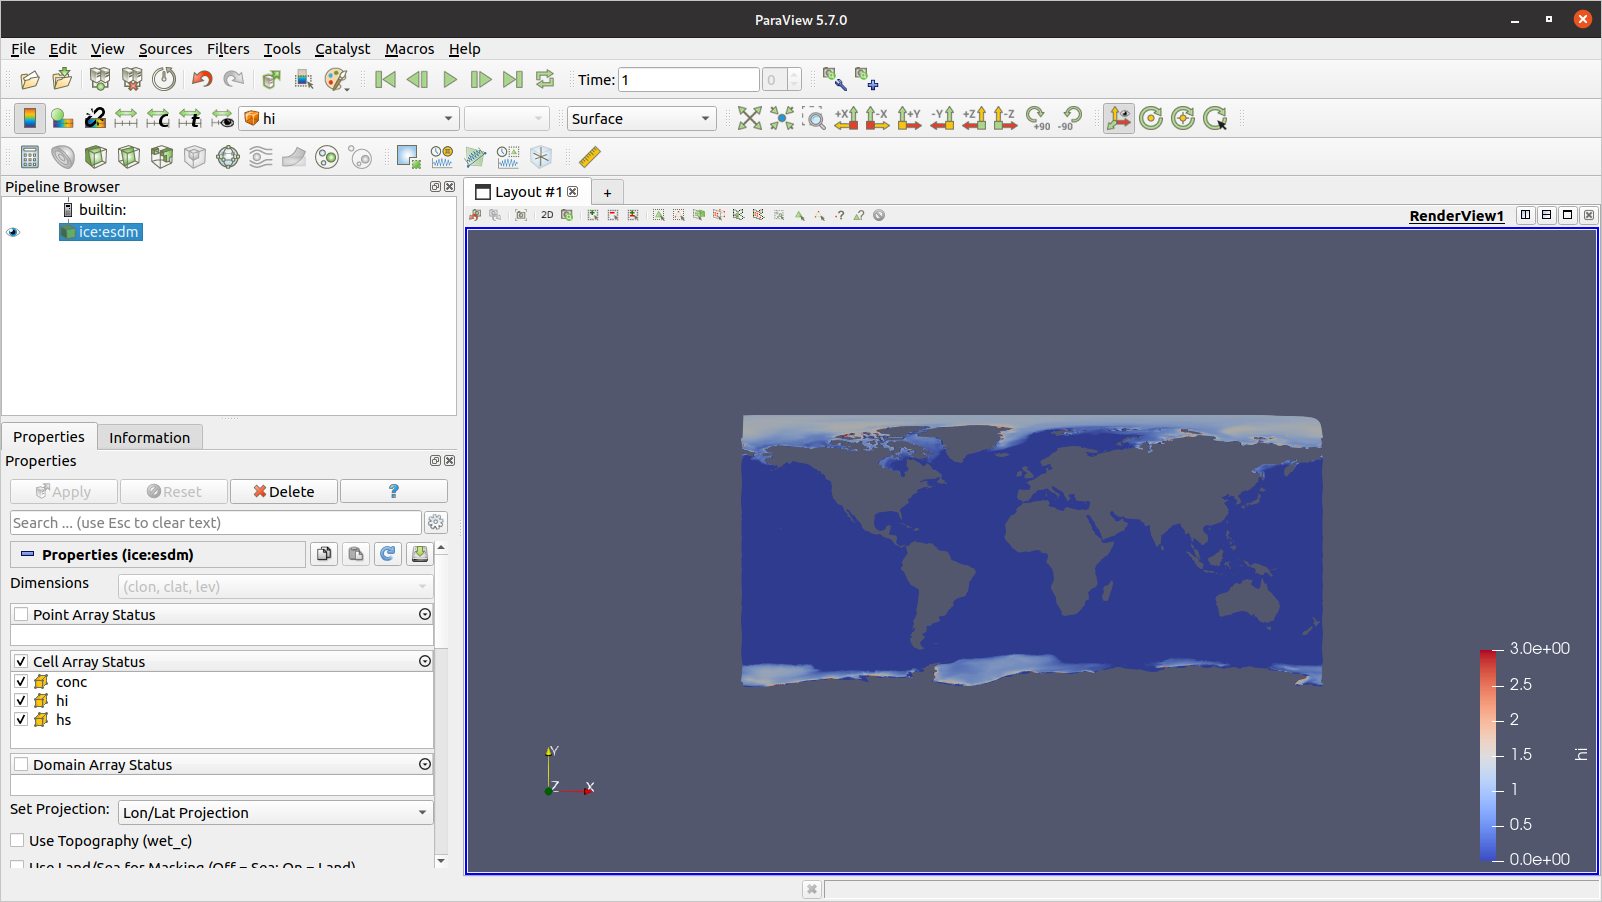
\includegraphics[width=\textwidth]{../figures/paraview.png}
  \end{center}
  \caption{Visualization of ice data set in Paraview. Data source is an ESDM file.}
  \label{fig:paraview}
\end{figure}
